% ##################################################################################################################
\section{Seoul}
\label{ch:seoul}
\hfill \textbf{Author:} Seungjae Lee, Atizaz Ali

% ##################################################################################################################
The MATSim model of Seoul Metropolitan was developed in 2012 as a result of long-term research collaboration between the University of Seoul (Prof.\ Seungjae Lee) \& ETH Zurich (Prof.\ Kay W.\ Axhausen). The model was updated on a yearly basis and the demand is generated based on 2012 Household Travel Survey Data (HHTSD). The brief statistics related to the demand (input) are summarized as follows. 

The study area covers the Seoul Metropolitan Area (Gyeonggi-do province with emphasis on Seoul Metro which comprises of 25 main administrative districts). Population Synthesizer was developed to generate the MATSim input demand based on HHTS 2012. Total population of SMA is 21.5 million; therefore, a 10\% sample was generated and simulated (2.15 million agents). A detailed network of nodes and links was generated capturing all the details (16'384 nodes and 32'768 links) for railways, highways, arterials, pedestrians, expressways and bus only lanes. EMME/2 network was converted to MATSim format. The 2012 Korean Transport Database was utilized to generate the transit schedules and vehicle definitions according to the bus types, railway and metro lines. Total number of routes is 1'317 (contains regional buses, inter-city buses, feeder line buses and metro lines etc.). In collaboration with Senozon AG, a more realistic door-door demand was generated in Seoul City in July 2014. Data source is the Korean GIS department.

In Seoul context, MATSim has been widely used for various research purposes for policy evaluation, see e.g., \citet[][]{KimEtAl_IJHE_2012, LeeAli_unpub_IWUTSCD_2014}.

A master's thesis is currently underway by this section's second author looking at transit demand generation and calibration using smart card data in SMA. The work is sequenced as follows. A video is available form the authors on request.
%
\begin{compactitem}
\item Data Mining (Trimming off non-useful data)
\item	Converting disaggregate transactions (OD’s )to individual trips and trip segments based on user ID
\item	Activities inference and assignment in SPSS database
\item	Generating transit demand (MATSim input format)
\item	Updated Transit Network \& Schedule for running the simulation
\item	Model calibration (in process)
\end{compactitem}
%
Moreover, MATSim tutorials are prepared for fall semester (2014) to help both undergrad and grad students at the Department of Transportation Engineering in getting working command at MATSim.

\createfigure%
{Seoul Scenario}%
{Seoul Scenario}%
{\label{fig:seoul}}%
{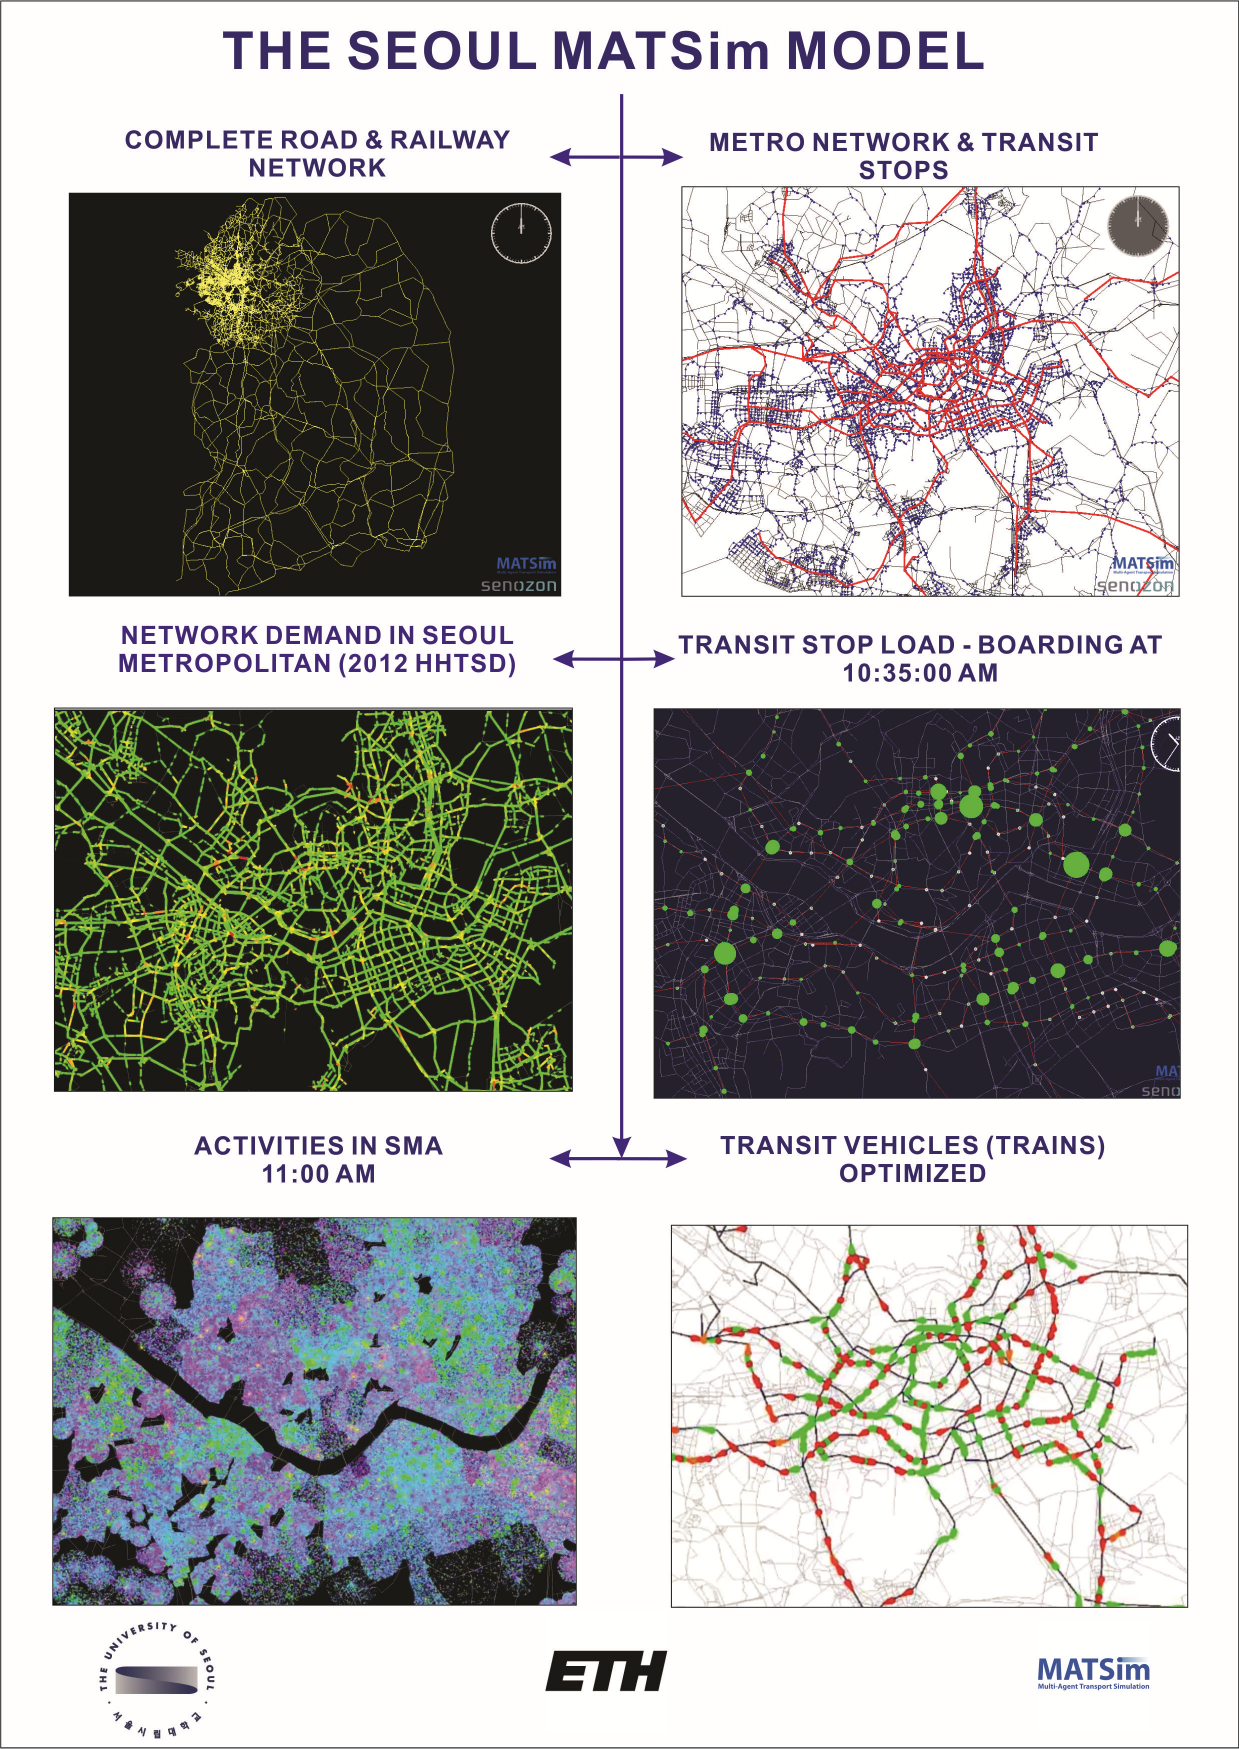
\includegraphics[width=0.99\textwidth, angle=0]{using/figures/seoul}}%
{}

% ##################################################################################################################
 
 
